\documentclass[12pt]{book}

%These tell TeX which packages to use.
\usepackage{array,epsfig}
\usepackage{amsmath}
\usepackage{amsfonts}
\usepackage{amssymb}
\usepackage{amsxtra}
\usepackage{amsthm}
\usepackage{mathrsfs}
\usepackage{color}
\usepackage{eurosym}
\usepackage{times}
\usepackage{enumitem}
\usepackage[normalem]{ulem}

%Here I define some theorem styles and shortcut commands for symbols I use often
\theoremstyle{definition}
\newtheorem{defn}{Definition}
\newtheorem{thm}{Theorem}
\newtheorem{cor}{Corollary}
\newtheorem*{rmk}{Remark}
\newtheorem{lem}{Lemma}
\newtheorem*{joke}{Joke}
\newtheorem{ex}{Example}
\newtheorem*{soln}{Solution}
\newtheorem{prop}{Proposition}

\newcommand{\lra}{\longrightarrow}
\newcommand{\ra}{\rightarrow}
\newcommand{\surj}{\twoheadrightarrow}
\newcommand{\graph}{\mathrm{graph}}
\newcommand{\bb}[1]{\mathbb{#1}}
\newcommand{\Z}{\bb{Z}}
\newcommand{\Q}{\bb{Q}}
\newcommand{\R}{\bb{R}}
\newcommand{\C}{\bb{C}}
\newcommand{\N}{\bb{N}}
\newcommand{\M}{\mathbf{M}}
\newcommand{\m}{\mathbf{m}}
\newcommand{\MM}{\mathscr{M}}
\newcommand{\HH}{\mathscr{H}}
\newcommand{\Om}{\Omega}
\newcommand{\Ho}{\in\HH(\Om)}
\newcommand{\bd}{\partial}
\newcommand{\del}{\partial}
\newcommand{\bardel}{\overline\partial}
\newcommand{\textdf}[1]{\textbf{\textsf{#1}}\index{#1}}
\newcommand{\img}{\mathrm{omega}}
\newcommand{\ip}[2]{\left\langle{#1},{#2}\right\rangle}
\newcommand{\inter}[1]{\mathrm{int}{#1}}
\newcommand{\exter}[1]{\mathrm{ext}{#1}}
\newcommand{\cl}[1]{\mathrm{cl}{#1}}
\newcommand{\ds}{\displaystyle}
\newcommand{\vol}{\mathrm{vol}}
\newcommand{\cnt}{\mathrm{ct}}
\newcommand{\osc}{\mathrm{osc}}
\newcommand{\LL}{\mathbf{L}}
\newcommand{\UU}{\mathbf{U}}
\newcommand{\support}{\mathrm{support}}
\newcommand{\AND}{\;\wedge\;}
\newcommand{\OR}{\;\vee\;}
\newcommand{\Oset}{\varnothing}
\newcommand{\st}{\ni}
\newcommand{\wh}{\widehat}

%Pagination stuff.
\setlength{\topmargin}{-.3 in}
\setlength{\oddsidemargin}{0in}
\setlength{\evensidemargin}{0in}
\setlength{\textheight}{9.in}
\setlength{\textwidth}{6.5in}
\pagestyle{empty}

\begin{document}

\begin{center}
{\Large DATA 221 \\  Homework 2  (rev 1)}\\
\textbf{W. Trimble}\\ %You should put your name here
Due: 11:59pm  Thursday 2023-01-19 
\end{center}

\vspace{0.2 cm}

\subsection*{   }

\begin{enumerate}

%\item
%Generate artificial data drawn from three classes, each a bivariate normal distribution, with the following parameters:
%
%\begin{tabular}{cccccccc}
%Class &  $x_0$  & $y_0$ & $\sigma_{xx}$ & $\sigma_{yy}$ & $\sigma_{xy}$ & n  \\
%Class A & -2 & 3 & 1 & 1.3 & 0.34 & 60\\
%Class B & 2 & -3 & 1 & 1.3 & 0.34 & 100 \\
%Class C & 0 & 0 & 0.7 & 0.7l &0.7 & 20 \\
%\end{tabular}

%In other words, draw a sample of 200 $(x,y)$ pairs, each with a label for class A, B, or C.
%Plot these on a scatter plot.

\item


\textbf{Naive Bayesian Spam Classifier}

Using the Kaggle "SMS Spam Collection Dataset," a collection of 5000 text messages, 13\% of which are labeled as spam, count the word usage for the spam messages and the word usages for the ham messages.

\texttt{https://www.kaggle.com/datasets/uciml/sms-spam-collection-dataset/}

Construct a function that scores new text messages by estimating $ {P (spam ) \over P(ham) } $.  Find the empirical word frequencies in the dataset $P (word | ham)$ and $P( word | spam ) $ 
for words that occur more than five times total in the dataset.
(This is somewhat ill-posed, since we have to assign a number to this probability ratio (even if it is 1) even for words that occur 0 times in the training data.)

As an ad-hoc data regularization approach, let us cap the maximum absolute value of the score that we will give to any word at 20; an utterance of 4 words that only appear in the spam corpus will get a score of 160000:1, and an utterance of 2 words that appear only in the ham corpus would get 1:400.  

\begin{enumerate}[label=(\alph*)]
\item
Use this to score all of the messages in the corpus described in 
Daniel R. O'Day and Ricardo A. Calix. "Text Message Corpus: Applying Natural Language Processing to Mobile Device Forensics," Proceedings of the Socio-Mobile Media Computing Workshop at IEEE International Conference on Multimedia and Expo, San Jose, USA. July 15 - 19, 2013, which is distributed at 

\texttt{https://web.archive.org/web/20130921042957/}

\texttt{http://cybersecurity.cit.purduecal.edu/content/dl/master\_corpus.txt}

\item
Plot the histogram of log-odds-scores for all the messages in the training set (disaggregated by Spam /not spam) and for all the log-odds scores for the messages in the American text-message corpus disaggregated by Incoming / Outgoing. 

Example code for tokenization will be provided.  This is a version of the loaded dice problem.

\end{enumerate}
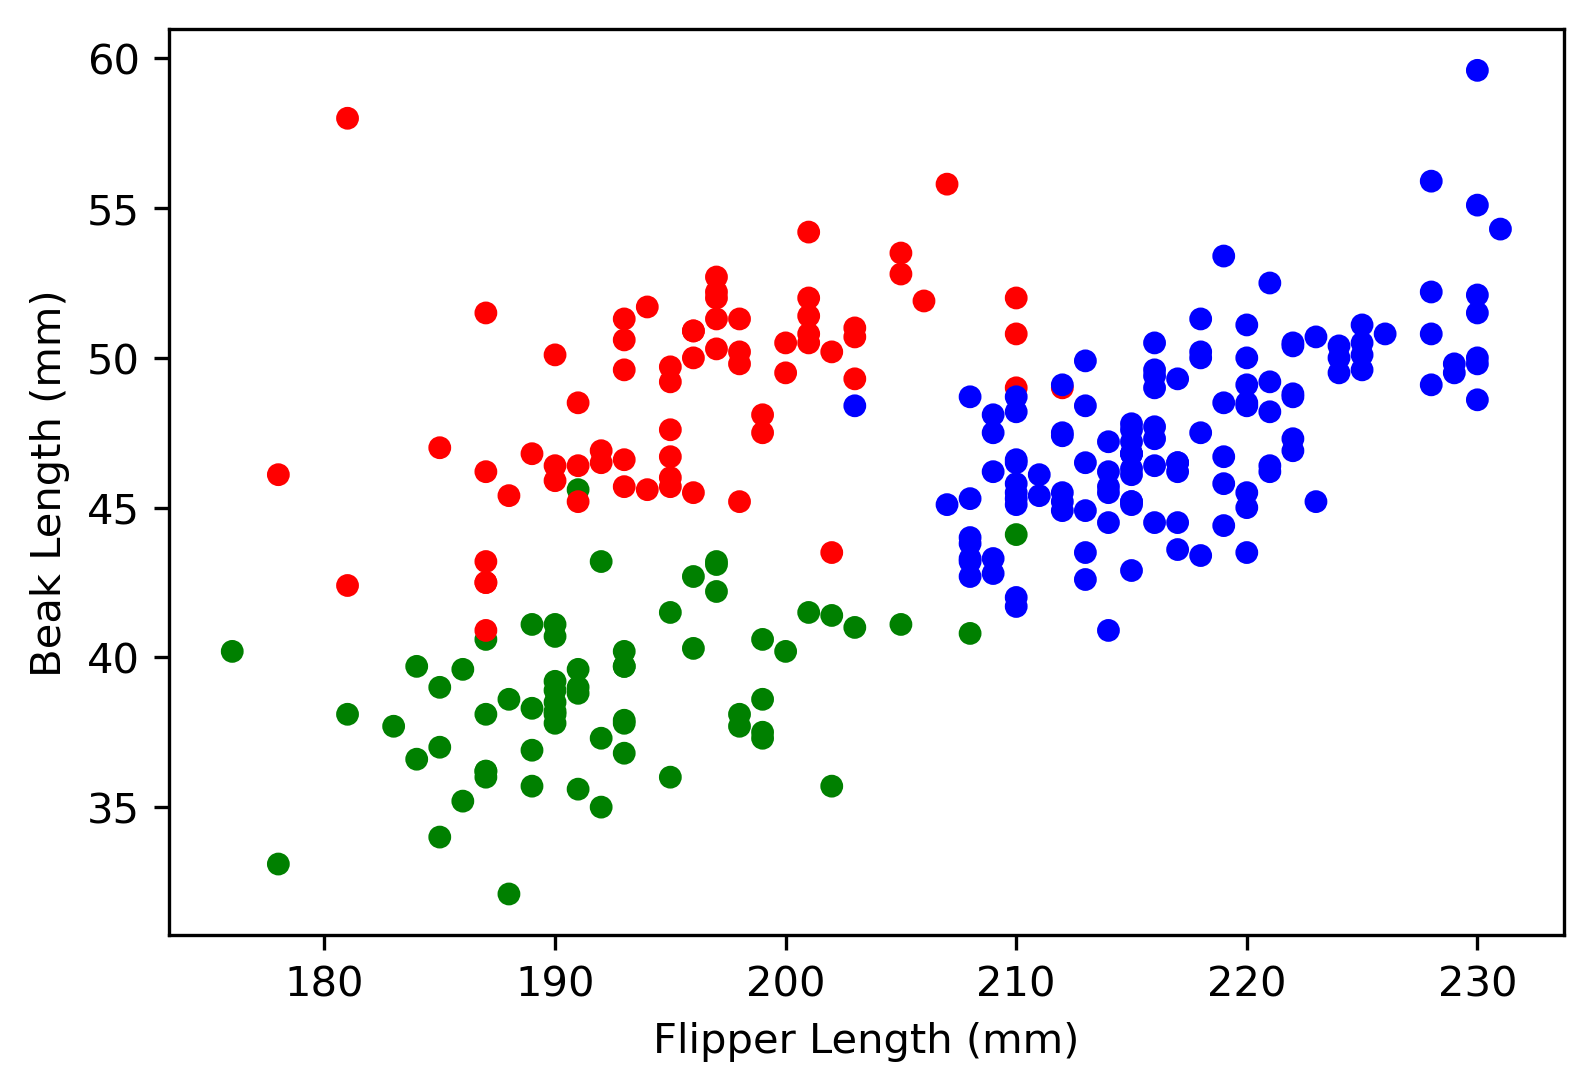
\includegraphics[width=4in]{PENGUIN.png}

\item\label{penguin}
\textbf{Linear Regression, Logistic Regression, and Linear Discriminant Analysis }
The Palmer penguins dataset has been split into a training set and a testing set. (n=265 and n=97).
This dataset has two "label" variables (sex and species) and four numerical "features."   We will try to classify penguins by species using three techniques that look at linear combinations of the feature vectors.
\begin{enumerate}[label=(\alph*)]
\item
Find linear regression coefficents for the indicator variables for species identity against the four-dimensional X.  
Plot the decision boundaries between the classes implied by the regression coefficients on top of the scatter plot.

\item
Find logistic regression coefficents for the indicator variables for species identity against the four-dimensional X. 
Plot the decision boundaries between the classes implied by the regression coefficients on top of the scatter plot.

\item
Find the class-conditional multivariate normal densities in four dimensions for each of the three penguin species using the training subset.
Plot the (quadratic) decision boundaries between penguin species on the scatter plot of flipper length vs. beak depth.

\item
Classify the test set by species and report the confusion matrix for one of the three classification methods above.

Here you can either plot the boundaries by finding the equations for the boundary or, if you find it easier, evaluate a classifier at a few hundred points on a 2d grid and plot a symbol on the graph indicating which regions of X get which classification; you can solve this with math or you can solve it numerically.  
\end{enumerate}


% \item\label{normal}
% \textbf{\sout{Bivariate normal properties NO NO NO }}
% Given a two-dimensional multivariate Gaussian distribution centered on (0,0) : 

%$$ \mathcal{N} ( \mathbf{x} ; \mathbf{\Sigma} ) =
%{ 1 \over( 2 \pi  ) }  
%{ 1 \over ( \sigma_{11}^2\sigma_{22}^2 - \sigma_{12}^2 )   }
%\exp  - { 1 \over 2} (
%\begin{bmatrix}
%x_0, & x_1
%\end{bmatrix}
%\begin{bmatrix}
%\sigma_{11}^2 & \sigma_{12}^2\\
%\sigma_{12}^2 & \sigma_{22}^2
%\end{bmatrix}^{-1}
%\begin{bmatrix}
%x_0 \\
%x_1
%\end{bmatrix} ) $$

%There are two linear combinations of $x_1$ and $x_2$ that maximize (minimize) the variance of the sums
%and at the same time make the two sums independent of each other.

%We can parameterize all possible sums of f $x_1$ and $x_2$  with $\theta$ : 

%$e_1 = \begin{pmatrix} 
%cos \theta \\
%sin \theta   \\
%\end{pmatrix} $ 
%and 
% $e_2 = \begin{pmatrix} 
%-sin \theta \\
%cos \theta   \\
%\end{pmatrix} $ 

%$$ z_1 = e_1 \cdot x $$
%and
%$$ z_2 = e_2 \cdot x $$
%Find the value of $\theta$ which makes the covariance between  $z_1$ and $z_2$ vanish.  Find the standard deviations of $z_1$ and $z_2$.



\end{enumerate}
\end{document}


